% =================================================================================================
% manual.tex — Guia rápido da Autosim para os participantes da pesquisa (formulário)
% Versão resumida dos Apêndices A–D da monografia.
%
% Compilar: pdflatex manual.tex
% =================================================================================================

\documentclass[11pt,a4paper]{article}

\usepackage[utf8]{inputenc}
\usepackage[T1]{fontenc}
\usepackage[brazilian]{babel}
\usepackage{lmodern}
\usepackage[margin=2cm]{geometry}
\usepackage{graphicx}
\usepackage{xcolor}
\usepackage{textcomp}
\usepackage{listings}
\usepackage{enumitem}
\usepackage[hidelinks]{hyperref}

\definecolor{acento}{RGB}{0,90,156}
\definecolor{fundo}{RGB}{243,245,248}

\lstset{
  basicstyle=\ttfamily\small,
  backgroundcolor=\color{fundo},
  frame=single,
  rulecolor=\color{acento!40},
  upquote=true,
  columns=fullflexible,
  keepspaces=true,
  showstringspaces=false,
  literate={-}{-}1,
  xleftmargin=4pt,
  xrightmargin=4pt,
}

% Título de cada passo
\newcommand{\passo}[2]{%
  \par\medskip
  {\large\bfseries\color{acento}#1.\ #2}\par\smallskip
}

\setlength{\parindent}{0pt}
\setlength{\parskip}{4pt}
\setlist{itemsep=2pt, topsep=2pt}

\begin{document}

\begin{center}
  {\LARGE\bfseries Autosim — Guia rápido}\\[4pt]
  Como abrir e simular um autômato em poucos minutos
\end{center}

A Autosim lê um arquivo de texto que descreve um autômato finito e mostra, em uma janela,
a simulação passo a passo. Ela não precisa ser instalada: basta baixar, extrair e rodar.

% -------------------------------------------------------------------------------------------------
\passo{1}{Baixe e extraia}

Acesse \url{https://github.com/KsBeckmann/autosim/releases/latest} e baixe o arquivo do seu
sistema:

\begin{itemize}
  \item \textbf{Windows:} \texttt{autosim-v1.0.3-windows-x86\_64.zip}
  \item \textbf{Linux:} \texttt{autosim-v1.0.3-linux-x86\_64.tar.gz}
  \item \textbf{macOS} (Apple M1, M2, M3\ldots): \texttt{autosim-v1.0.3-macos-aarch64.tar.gz}
\end{itemize}

Extraia o arquivo (botão direito $\rightarrow$ \emph{Extrair tudo} ou \emph{Extrair aqui}).
Vai aparecer uma pasta com o programa \texttt{autosim} e uma pasta \texttt{examples}, com
autômatos prontos.

% -------------------------------------------------------------------------------------------------
\passo{2}{Abra um terminal dentro da pasta}

A Autosim é aberta por um comando no terminal. \textbf{Dar dois cliques no programa não
funciona}, porque ele precisa saber qual arquivo abrir.

\begin{itemize}
  \item \textbf{Windows:} abra a pasta extraída, clique na barra de endereço (onde aparece o
  caminho da pasta), apague o que estiver escrito, digite \texttt{cmd} e aperte
  \textbf{Enter}.
  \item \textbf{Linux e macOS:} abra o Terminal, digite \texttt{cd} seguido de um espaço,
  arraste a pasta extraída para dentro da janela do terminal e aperte \textbf{Enter}.
\end{itemize}

% -------------------------------------------------------------------------------------------------
\passo{3}{Rode um exemplo}

Digite o comando abaixo e aperte \textbf{Enter}:

\textbf{Windows:}
\begin{lstlisting}
.\autosim.exe -p examples\example1.asl
\end{lstlisting}

\textbf{Linux e macOS:}
\begin{lstlisting}
./autosim -p examples/example1.asl
\end{lstlisting}

\textbf{Se o sistema bloquear o programa:}
\begin{itemize}
  \item \textbf{Windows:} no aviso ``O Windows protegeu o computador'', clique em
  \emph{Mais informações} $\rightarrow$ \emph{Executar assim mesmo}.
  \item \textbf{macOS:} rode uma vez \texttt{xattr -d com.apple.quarantine autosim} e
  tente de novo.
\end{itemize}

% -------------------------------------------------------------------------------------------------
\newpage
\passo{4}{Use a janela}

\begin{center}
  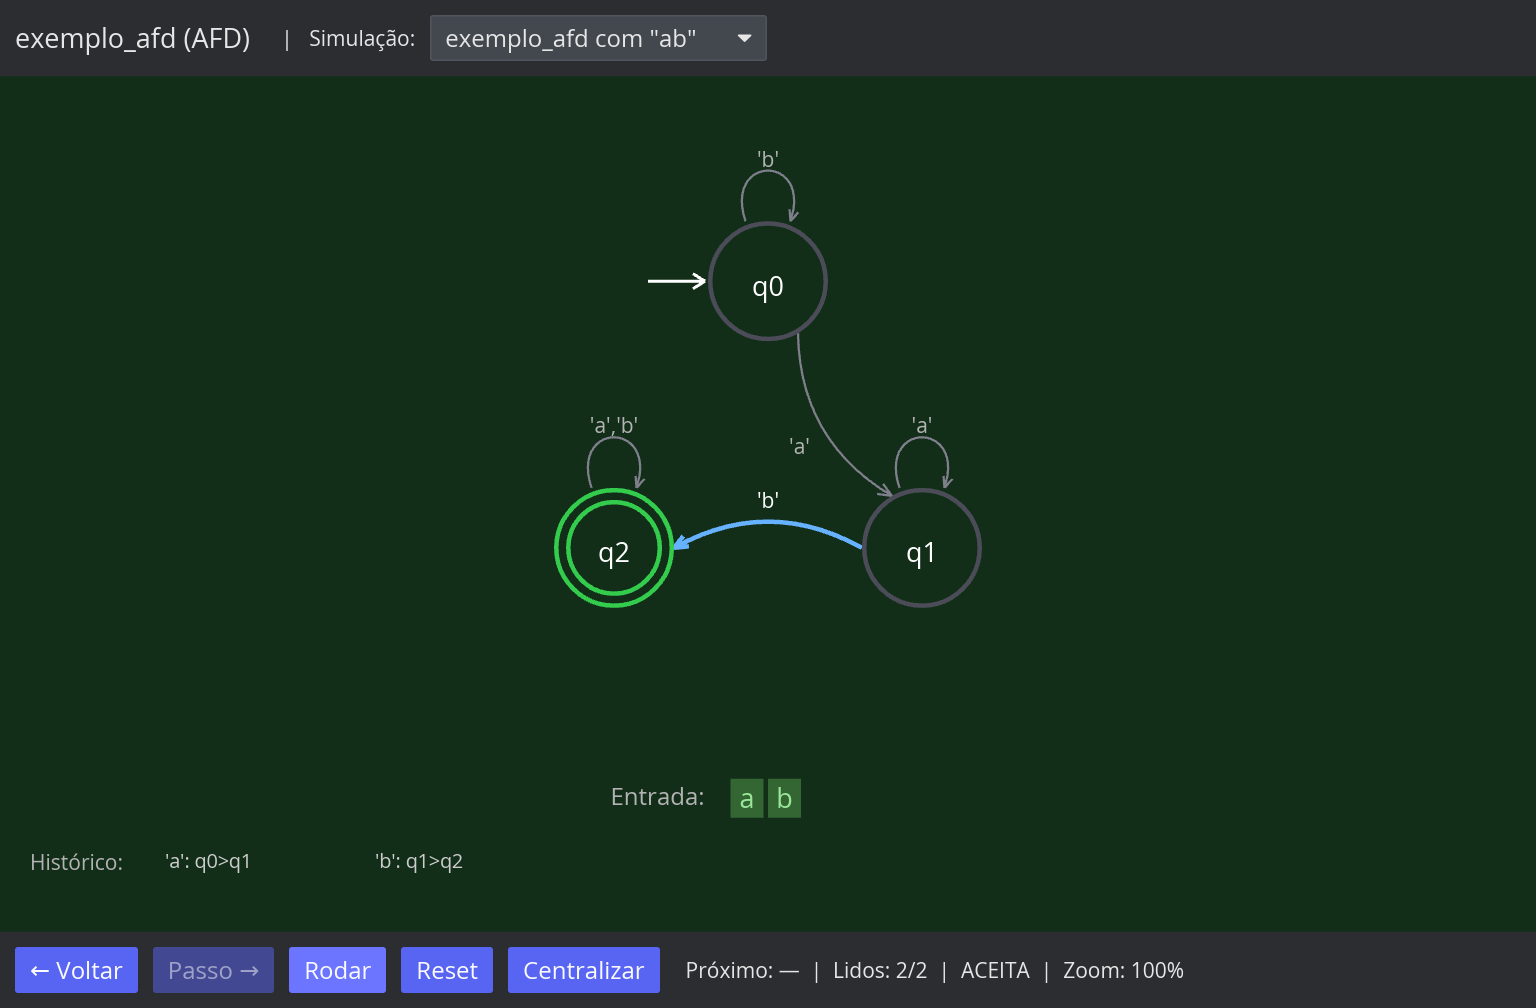
\includegraphics[width=0.82\textwidth]{img/interface_simulacao_aceita.png}
\end{center}

\begin{itemize}
  \item \textbf{No topo}, em \emph{Simulação}, escolha qual cadeia simular. O arquivo
  \texttt{example1.asl} tem quatro.
  \item \textbf{Passo $\rightarrow$} lê o próximo símbolo da cadeia e mostra a transição
  usada. \textbf{$\leftarrow$ Voltar} desfaz o último passo.
  \item \textbf{Rodar} faz a simulação andar sozinha; \textbf{Reset} recomeça do início.
  \item No fim, o estado fica \textcolor{green!50!black}{\textbf{verde}} e aparece
  \textbf{ACEITA} se a cadeia é aceita, ou fica \textcolor{red!70!black}{\textbf{vermelho}}
  com \textbf{REJEITA} se não é.
  \item Arraste o diagrama com o \emph{mouse} para movê-lo e use a rodinha para dar
  \emph{zoom}. \textbf{Centralizar} volta à posição original.
\end{itemize}

Experimente também \texttt{examples/afn\_epsilon.asl}, um AFN com transições vazias
($\varepsilon$).

% -------------------------------------------------------------------------------------------------
\passo{5}{Veja uma mensagem de erro}

Feche a janela e rode um arquivo que tem um erro proposital:

\textbf{Windows:}
\begin{lstlisting}
.\autosim.exe -p examples\sema_nondeterministic.asl
\end{lstlisting}

\textbf{Linux e macOS:}
\begin{lstlisting}
./autosim -p examples/sema_nondeterministic.asl
\end{lstlisting}

Desta vez a janela não abre: o erro aparece no terminal. A primeira linha diz qual é o
problema, entre colchetes vem o arquivo, a linha e a coluna, e os rótulos coloridos apontam
o trecho exato do código. Neste exemplo, um AFD tem duas transições saindo de \texttt{q0}
com o mesmo símbolo, o que não é permitido em um AFD.

% -------------------------------------------------------------------------------------------------
\newpage
\passo{6}{(Opcional) Escreva o seu autômato}

Crie um arquivo de texto com a extensão \texttt{.asl} na mesma pasta do programa e rode-o
como no passo 3, trocando o nome do arquivo. No Bloco de Notas do Windows, ao salvar,
escolha \emph{Tipo: Todos os arquivos}, senão o arquivo vira \texttt{.asl.txt}. Exemplo de um AFD que aceita as cadeias
sobre \{a, b\} que terminam em \texttt{b}:

\begin{lstlisting}
alfabeto { 'a', 'b' }

automato AFD termina_em_b {
    estados { q0, q1 }
    inicial q0
    finais { q1 }
    transicoes {
        q0 -> q0 com 'a'
        q0 -> q1 com 'b'
        q1 -> q0 com 'a'
        q1 -> q1 com 'b'
    }
}

simular termina_em_b com "aab"   // aceita
simular termina_em_b com "ba"    // rejeita
\end{lstlisting}

Regras básicas: cada símbolo fica entre aspas simples (\texttt{'a'}); a cadeia simulada
fica entre aspas duplas (\texttt{\string"ab\string"}); em um AFN, \texttt{eps} indica uma transição vazia;
e o que vem depois de \texttt{//} é comentário.

\vfill
\begin{center}
  \colorbox{acento!10}{\parbox{0.9\textwidth}{\centering\smallskip
  \textbf{Pronto!} Agora volte ao formulário e responda às perguntas.\\
  Obrigado por participar!\smallskip}}
\end{center}

\end{document}
